\documentclass{standalone}
\usepackage{tikz}
\usepackage{pgfplots}
\pgfplotsset{compat=1.18}
\begin{document}

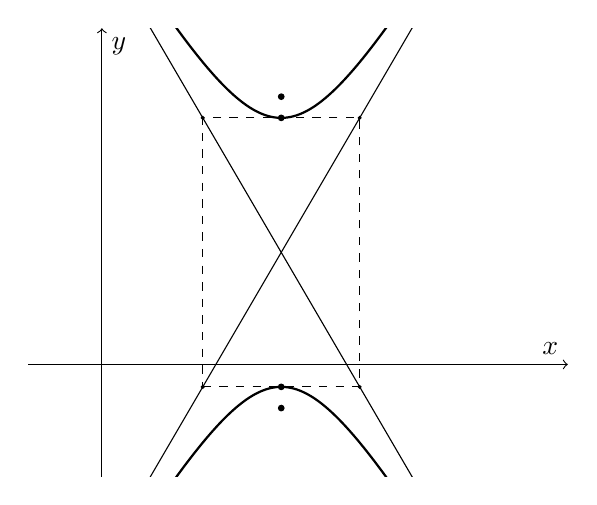
\begin{tikzpicture}[scale=1]
\begin{axis}[
    xmin=-0.5, xmax=18,
    ymin=-5, ymax=15,
    axis lines=middle,
    axis line style={->},
    ticklabel style={font=\tiny},
    axis equal,
    xtick=\empty,%{-8,-7,-6,-5,-4,-3,-2,-1,0,1,2,3,4,5,6,7,8},
    ytick=\empty,%{-5,-4,-3,-2,-1,0,1,2,3,4,5},
    xticklabels=\empty,
    yticklabels=\empty,
    xlabel={$x$},
    ylabel={$y$}
]

% Parameters
\def\a{3.5}
\def\b{6}
\pgfmathsetmacro{\c}{sqrt(\a*\a + \b*\b)}

% Translation
\def\h{8}   % shift right
\def\k{5}   % shift up

% Hyperbola
\addplot [domain=-1.5:1.5, samples=200, thick] 
    ({\h + \a*sinh(x)}, {\k + \b*cosh(x)});
\addplot [domain=-1.5:1.5, samples=200, thick] 
    ({\h - \a*sinh(x)}, {\k - \b*cosh(x)});

% Asymptotes
\addplot [domain=-8:15] {\k + (\b/\a)*(x-\h)};
\addplot [domain=-8:15] {\k - (\b/\a)*(x-\h)};

% Conjugate rectangle
\addplot [dashed] coordinates {
    (\h-\a,\k-\b)
    (\h+\a,\k-\b)
    (\h+\a,\k+\b)
    (\h-\a,\k+\b)
    (\h-\a,\k-\b)
};

% Foci
\filldraw (axis cs:\h,\k+\c) circle (1pt);
%\node[above] at (axis cs:\h+\c,\k) {$c$};
\filldraw (axis cs:\h,\k-\c) circle (1pt);
%\node[above] at (axis cs:\h-\c,\k) {$-c$};

% Vertices
\filldraw (axis cs:\h,\k+\b) circle (1pt);
%\node[above] at (axis cs:\h+\a,\k) {$a$};
\filldraw (axis cs:\h,\k-\b) circle (1pt);
%\node[above] at (axis cs:\h-\a,\k) {$-a$};

% Rectangle corners
\filldraw (axis cs:\h-\a,\k-\b) circle (0.5pt);
\filldraw (axis cs:\h+\a,\k+\b) circle (0.5pt);
\filldraw (axis cs:\h-\a,\k+\b) circle (0.5pt);
\filldraw (axis cs:\h+\a,\k-\b) circle (0.5pt);

% Labels
%\node[left] at (axis cs:\h,\k+\b) {$b$};
%\node[left] at (axis cs:\h,\k-\b) {$-b$};

% Diagonal segment
%\draw[<->, thick] 
%(axis cs:\h,\k) -- (axis cs:\h+\a,\k+\b) node[midway, above] {$c$};

\end{axis}
\end{tikzpicture}


\end{document}